\documentclass{standalone}
\usepackage{tikz}
\begin{document}


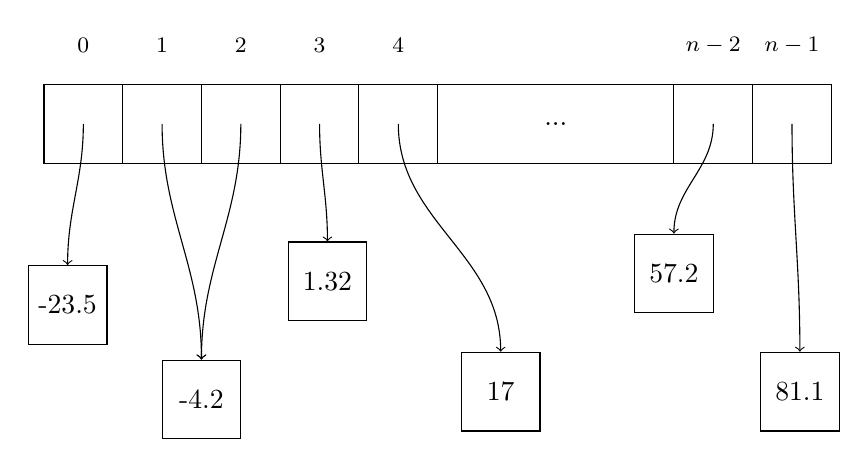
\begin{tikzpicture}
\node[minimum size=1cm,draw] at (0,0) {};
\node[minimum size=1cm,draw] at (1,0) {};
\node[minimum size=1cm,draw] at (2,0) {};
\node[minimum size=1cm,draw] at (3,0) {};
\node[minimum size=1cm,draw] at (4,0) {};
\node[minimum size=1cm,minimum width=3cm,draw] at (6,0) {...};
\node[minimum size=1cm,draw] at (8,0) {};
\node[minimum size=1cm,draw] at (9,0) {};

\node[minimum size=1cm,draw] (a) at (-0.2,-2.3) {-23.5};
\node[minimum size=1cm,draw] (b) at (1.5,-3.5) {-4.2};
\node[minimum size=1cm,draw] (c) at (3.1,-2.0) {1.32};
\node[minimum size=1cm,draw] (d) at (5.3,-3.4) {17};
\node[minimum size=1cm,draw] (e) at (7.5,-1.9) {57.2};
\node[minimum size=1cm,draw] (f) at (9.1,-3.4) {81.1};

\draw[->] (0,0) to [out=270,in=90] (a);
\draw[->] (1,0) to [out=270,in=90] (b);
\draw[->] (2,0) to [out=270,in=90] (b);
\draw[->] (3,0) to [out=270,in=90] (c);
\draw[->] (4,0) to [out=270,in=90] (d);
\draw[->] (8,0) to [out=270,in=90] (e);
\draw[->] (9,0) to [out=270,in=90] (f);

\node at (0,1) {\footnotesize 0};
\node at (1,1) {\footnotesize 1};
\node at (2,1) {\footnotesize 2};
\node at (3,1) {\footnotesize 3};
\node at (4,1) {\footnotesize 4};
\node at (8,1) {\footnotesize $n-2$};
\node at (9,1) {\footnotesize $n-1$};
\end{tikzpicture}


\end{document}
